% Slide Preamble
\documentclass[svgnames]{beamer}
\usepackage[english]{babel}
\usepackage[utf8]{inputenc}
\usepackage{calc}
\usepackage[absolute,overlay]{textpos}
\usepackage{graphicx}
\usepackage{subfig}
\usepackage{amsmath}
\usepackage{amsfonts}
\usepackage{amsthm}
\usepackage{mathtools}
\usepackage{listings}
\usepackage{standalone}
\usepackage{comment}
\usepackage{bbding}
\usepackage[plain]{algorithm}
\usepackage{caption}
\usepackage[noend]{algpseudocode} % needed for: algorithm pseudocode
\usepackage{MnSymbol,wasysym}

\setbeamertemplate{navigation symbols}{} % remove navigation symbols
\mode<presentation>{\usepackage{class/beamerthemetud}}

% BIB SETTINGS
\usepackage[backend=bibtex,firstinits=true,maxnames=30,maxcitenames=20,url=false,style=authoryear]{biblatex}
\bibliography{references}
\setlength\bibitemsep{0.3cm} % space between entries in the reference list
\renewcommand{\bibfont}{\normalfont\scriptsize}
\setbeamerfont{footnote}{size=\tiny}
\renewcommand{\cite}[1]{\footnote<.->[frame]{\fullcite{#1}}}

\usepackage{tikz,tcolorbox}
\usetikzlibrary{decorations.pathreplacing} 
\usetikzlibrary{arrows,decorations.pathreplacing,decorations.pathmorphing,decorations.footprints,
	fadings,calc,trees,mindmap,shadows,decorations.text,patterns,positioning,shapes,matrix,fit}
\usepackage{stmaryrd}
\input{class/tikz_defs}

\begin{document}

% title page

\def\TITLE	{\textbf{\huge Virtualization (Task Merging) \\ Design \& Implementation}}		% on the 
%first slide
\def\SHORTTITLE		{Virtualization}										% 
%on 
%``testatine''
\def\AUTHOR			{-}						% }
%on the 
%first slide
\def\SHORTAUTHOR	{-}								% on 
%``testatine''
\def\INSTITUTE		{Embedded Software Group -- Delft University of Technology, 
The Netherlands}							% on the first slide
\def\SHORTINSTITUTE	{TU Delft}													
% on ``testatine''

\title		[\SHORTTITLE]		{\TITLE}
\author		[\SHORTAUTHOR]		{\AUTHOR}
\date		{8 February 2017}									% keep empty 
%for no dates
\institute	[\SHORTINSTITUTE]	{\INSTITUTE}


{
\setbeamertemplate{footline}{\usebeamertemplate*{no footline}}

\begin{frame}
	\titlepage	
%	\begin{center}
%		\begin{tabular}{cc}
%			\includegraphics[height = 1.0cm]{images/logo_es} &
%			\includegraphics[height = 2cm]{images/logo_color}
%		\end{tabular}
%	\end{center}
	%
	\centering
	\includegraphics[height = 1.0cm]{images/logo_es}
	\vspace{0.3cm}
	%
	\begin{center}
	\end{center}
\end{frame}
}


{
	\setbeamertemplate{footline}{\usebeamertemplate*{footline}}
}

%---------------------------------------------------------------------------

\begin{frame}{\textbf{Virtualization --- Motivation}}
	\begin{alertblock}{\textbf{FRAM Write}}
		\begin{itemize}
			\item Almost twice more expensive than SRAM write.
		\end{itemize}	
	\end{alertblock}	
	
	\centering
	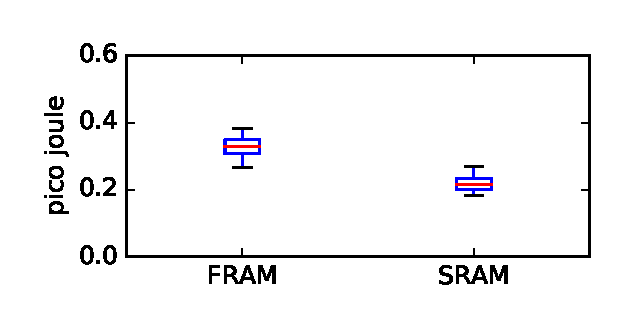
\includegraphics[scale=0.5]{images/fram_write.eps}
	
	
	\begin{block}{\textbf{Problem Statement}}
		\begin{itemize}
			\item How to \textbf{postpone} FRAM access (commit) operations to reduce energy overhead? 	
			\begin{itemize}
				\item The gained energy will be used for \textbf{more computation} 
				\item E.g. more tasks will be executed in task-based programs --- in turn, the total program execution time will be reduced	
				\begin{itemize}
					\item Portability: different super-capacitor sizes will be used efficiently	
				\end{itemize}
			\end{itemize}		
		\end{itemize}	
	\end{block}
	
\end{frame}

%---------------------------------------------------------------------------

\begin{frame}{\textbf{Task-based Control Flow}}
	
	\begin{itemize}
		\item e.g. Chain\cite{colin2016chain} 
		\begin{itemize}
			\item no checkpointing -- keep track of the current task 
			\item pipelined channels -- maintain the consistency of 
			FRAM
			\item seperate inputs from outputs -- idempotency
		\end{itemize}
		
	\end{itemize}
	
	\begin{columns}		
		
		\column{.40\textwidth}
		\centering
		\includegraphics[scale=0.10]{images/chain.png}\\
		
		\column{.56\textwidth}
		\begin{block}{\textbf{Drawbacks}}
			\begin{itemize}
				\item outputs are committed \textbf{at the end} of each task
				\begin{itemize}
					\item \textbf{Commit} operation, in turn FRAM access (in particular write), is \textbf{expensive}
				\end{itemize}
				\item \textbf{multi-versioning} of variables --- memory overhead
				\begin{itemize}	
					\item increased number of FRAM operations
				\end{itemize}
			\end{itemize}	
		\end{block}
		
	\end{columns}
	
\end{frame}


%---------------------------------------------------------------------------


\begin{frame}{\textbf{Details - Virtualization of Chain -I}}
	
	\begin{columns}		
		
		\column{.70\textwidth}
		\begin{itemize}
			\item If all output channels are connected to and the transition path is only to the \textbf{next task}, virtualization is \textbf{easy}! 
			\item Example: no need to commit \texttt{Channel (1)} and \texttt{Channel (2)} since their values are already consumed to output \texttt{Channel (3)}.
		\end{itemize}
		
		\column{.40\textwidth}
		\center
		\includegraphics[scale=0.50]{images/chain-virtualization.pdf}
	\end{columns}	
		
		\begin{block}{\textbf{Strategy}}
			\begin{itemize}
				\item Postpone commit inside the \textbf{virtualization window} using corresponding \textbf{soft-channels} in SRAM
				\item \textbf{Hard-commit} only the channel input of the last task 
				\item If power-interrupted, go to the first task of the window
			\end{itemize}	
		\end{block}
			
\end{frame}

%---------------------------------------------------------------------------


\begin{frame}{\textbf{Details - Virtualization of Chain -II}}
	
	\begin{columns}		
		
		\column{.77\textwidth}
		\begin{itemize}
			\item What if the channel connections and transition paths are \textbf{divergent}? 
			\begin{itemize}
				\item Example: \texttt{Channel (3)}, \texttt{Channel (4)} and \texttt{Channel (5)} \textbf{must} committed to FRAM ---\textbf{hard-channels}
				\item \texttt{Channel (1)} and \texttt{Channel (2)} are in SRAM---\textbf{soft-channels}
				\item \texttt{Channel (6)} should be \textbf{read} from FRAM---hard-channel
			\end{itemize}
		\end{itemize}
		
		\column{.35\textwidth}
		\includegraphics[scale=0.50]{images/chain-virtualization-II.pdf}
	\end{columns}	
	
	\begin{block}{\textbf{Drawbacks}}
		\begin{itemize}
			\item The static \textbf{task-graph} and the \textbf{dynamic} transition path should be used at \textbf{run-time} to decide which channels need to be hard or soft
		\end{itemize}	
	\end{block}

	\begin{alertblock}{\textbf{Not Feasible}}
	\begin{itemize}
		\item Due to \textbf{loops} in task graph, e.g. self-channels, and \textbf{multi-versioning} ruins virtualization.
	\end{itemize}	
\end{alertblock}
	
\end{frame}
%---------------------------------------------------------------------------


\begin{frame}{\textbf{Case Study - Virtualization of ALPACA -I}}
	
		\centering
		\includegraphics[scale=0.3]{images/alpaca-privatization.png} \\
Only variables with W-A-R dependencies are protected in ALPACA.
		

	
	\begin{block}{\textbf{Challanges}}
		\begin{itemize}
			\item Variables without W-A-R dependencies are directly read from/written to FRAM 
			\item \textbf{Solution:} Use \textbf{SRAM buffer} and commit later---Reduced FRAM access
		\end{itemize}	
	\end{block}
	
\end{frame}

%---------------------------------------------------------------------------


\begin{frame}{\textbf{Case Study - Virtualization of ALPACA -II}}
	
	\begin{columns}		
	
	\column{.65\textwidth}
	\begin{itemize}
		\item Merged tasks might introduce new W-A-R dependencies ---at \textbf{run-time}!
		\item How to \textbf{dynamically} keep-track of the privitization of the W-A-R dependencies? ---\textbf{too much overhead!}
		\begin{itemize}
			\item Alpaca does not privatize \texttt{x}, \texttt{y} and \texttt{z}; they are directly written to FRAM. 
			\item We need software implementation of Clank :)
		\end{itemize}
	\end{itemize}
	
	\column{.45\textwidth}
	\includegraphics[scale=0.7]{images/alpaca-war.pdf}
\end{columns}	

\begin{alertblock}{\textbf{Conclusions}}
	\begin{itemize}
		\item We need to \textbf{eliminate} privatization so that tasks can operate on SRAM efficiently.
		\item Not Feasible with ALPACA, requires fundamental design changes.
	\end{itemize}	
\end{alertblock}
	
\end{frame}

%---------------------------------------------------------------------------


\begin{frame}{\textbf{Virtualization with SRAM Buffer-I}}
	\begin{columns}		
		
	\column{.41\textwidth}
	\begin{itemize}
		\item Version \textbf{task-shared} variables in FRAM
		\item A \textbf{fixed-sized} SRAM buffer for virtual operations
		\item Two-phase commit at the end of the \textbf{virtual task}.
	\end{itemize}
	
	
		\column{.70\textwidth}
\includegraphics[scale=0.5]{images/sram-buffer.pdf}	
\end{columns}
	
	\begin{block}{\textbf{Overhead}}
		\begin{itemize}
			\item \texttt{get} and \texttt{set} operations require \textbf{search} in SRAM cache
			\item Example: The presented task in Alpaca will have 4 FRAM write operations - We will have 6 + SRAM search overhead!
		\end{itemize}	
	\end{block}
	
\end{frame}


%---------------------------------------------------------------------------


\begin{frame}{\textbf{Virtualization with SRAM Buffers-II}}
	\begin{columns}		
		
		\column{.50\textwidth}
		\begin{itemize}
			\item We did not observe any benefit, even worse!
			\item CPU is the main burden in energy consumption --- Search operations dominate FRAM write!
		\end{itemize}
		
		
		\column{.50\textwidth}
		\includegraphics[scale=0.3]{images/sram-sw-buffer.pdf}	
	\end{columns}

	
	\begin{alertblock}{\textbf{Problem}}
	\begin{itemize}
		\item How to eliminate SRAM Cache search operation? 
		\item How to minimize commit overhead?
	\end{itemize}	
	\end{alertblock}

	
\end{frame}

%---------------------------------------------------------------------------


\begin{frame}{\textbf{Virtualization with DMA Support-I}}
	\begin{columns}		
		
		\column{.60\textwidth}
		\begin{itemize}
			\item Exploit hardware that is found in almost every CPU architecture
			\item Copying block of words from/to SRAM-FRAM and FRAM-FRAM is very \textbf{cheap} and \textbf{scalable} with DMA!
		\end{itemize}
		
		
		\column{.42\textwidth}
		\includegraphics[scale=0.25]{images/dmaSize.eps}\\			
		\includegraphics[scale=0.25]{images/energyConsumptionDMA_SW.eps}	
	\end{columns}
	
	
	\begin{alertblock}{\textbf{Problem}}
		\begin{itemize}
			\item How to eliminate SRAM Cache search operation? 
			\item How to minimize commit overhead?
		\end{itemize}	
	\end{alertblock}
	
	
\end{frame}
%---------------------------------------------------------------------------


\begin{frame}{\textbf{Virtualization with DMA Support-II}}
	\begin{columns}		
		
		\column{.41\textwidth}
		\begin{itemize}
			\item Version all \textbf{task-shared} variables in FRAM
			\item Bring all to SRAM buffer for virtual operations
			\item Two-phase commit at the end of the \textbf{virtual task}.
		\end{itemize}
		
		
		\column{.70\textwidth}
		\includegraphics[scale=0.5]{images/dma.pdf}	
	\end{columns}
	
	\begin{block}{\textbf{Feasibility}}
		\begin{itemize}
			\item Perform all these operations using DMA!
			\item All task-shared variables have a copy in SRAM, \textbf{no search}!
		\end{itemize}	
	\end{block}
	
\end{frame}

%---------------------------------------------------------------------------


\begin{frame}{\textbf{Virtualization with DMA Support-III}}
	\center
	\includegraphics[scale=0.27]{images/executionTime-eps-converted-to}	
	\includegraphics[scale=0.27]{images/virtualTaskSize-eps-converted-to}
	
\end{frame}

%---------------------------------------------------------------------------


\begin{frame}{\textbf{Virtualization with DMA Support-Limitations-I}}
	
	\begin{itemize}
			\item The size of the task-shared variables, in turn the size of SRAM Cache is bounded with the \textbf{SRAM size} in the platform.
			\begin{itemize}
				\item The number of channels is directly limited with the FRAM size in Chain
				\item The size of the commit list in Alpaca, i.e. the number of variables with W-A-R dependency inside a task, is limited with the FRAM.
			\end{itemize}
	\end{itemize}

\centering
\begin{block}{}
	\centering
	\begin{tabular}{ l c | c | c }
	& VIPOS & Chain & Alpaca \\
	\hline
	\textbf{Limited with} & SRAM-size & FRAM-size & FRAM-size
\end{tabular}
\end{block}
	
\end{frame}
%---------------------------------------------------------------------------


\begin{frame}{\textbf{Virtualization with DMA Support-Limitations-II}}

\begin{itemize}

		\item The cost of start-up and commit operations increase with \textbf{the size of the task-shared variables}
		\begin{itemize}
			\item But this comes with the elimination of the search operations in SRAM cache and selective commit
			\item DMA cost increases linearly but very slowly.
		\end{itemize}
\end{itemize}	
All these limitations are paid in order to benefit from virtualization.

\end{frame}
%---------------------------------------------------------------------------

\begin{frame}{\textbf{What is next?}}
	
	\begin{itemize}
		\item How to get rid of flush in/out all task-shared global variables?
		\begin{itemize}
			\item Very difficult, how?
		\end{itemize} 
		\item Development and evaluation of several task-merging algorithms, i.e. \textbf{ virtualization scheduler}
		\begin{itemize}
			\item This will be one of the core sections of the paper!
		\end{itemize}
		\item Automatic "taskification"
		\begin{itemize}
			\item This will be one of the core sections of the paper!
		\end{itemize}
	\end{itemize}
	
\end{frame}

%---------------------------------------------------------------------------

\begin{frame}{\textbf{The structure of the article-I}}
	
	\begin{itemize}
		\item \textbf{Introduction}
		\begin{itemize}
			\item Motivation---FRAM access, in turn commit cost, need for the virtualization
			\item Problem statement
			\item Challenges---Why it is difficult to modify state of the art solutions to support virtualization?
			\item Our solution and contributions---Sketch of our solution and attractive results
		\end{itemize}
		\item \textbf{Challenges}
	\begin{itemize}
		\item Intermittent programming with checkpointing and task-based control flow
		\item Stress the problem of dynamic merging of the tasks, its feasibility with the state of the art solutions, e.g. Chain, InOS, Alpaca...
	\end{itemize}
	
		\item \textbf{Virtualization: Dynamic Merging of Tasks}
		\begin{itemize}
			\item Introduce the concept, requirements
			\item Design objectives
			\item Introduce the infrastructure here
		\end{itemize}
	\end{itemize}
	
\end{frame}

%---------------------------------------------------------------------------

\begin{frame}{\textbf{The structure of the article-II}}
	
	\begin{itemize}
		\item \textbf{Virtualization Scheduler: The Algorithms}
		\begin{itemize}
			\item Introduce the task-merging strategies that work on the infrastructre in the previous section
			\item Analysis of the algorithms
			\item Maybe some simulations
		\end{itemize}
		\item \textbf{Implementation and Evaluation}
		\begin{itemize}
			\item Introduce the implementation details
			\item Test-bed setup
			\item Experimental results
			\item Simulations
		\end{itemize}
		\item \textbf{Related Work}
		\item \textbf{Conclusions}
	\end{itemize}
	
\end{frame}


\end{document}
